\documentclass{article}
\usepackage[T1]{fontenc}
\usepackage{lmodern}
\usepackage{graphicx}
\usepackage{amsmath,amssymb}
\usepackage[a4paper,margin=2cm]{geometry}
\usepackage[absolute,overlay]{textpos}
\setlength{\TPHorizModule}{1mm}
\setlength{\TPVertModule}{1mm}
\usepackage[indonesian]{babel}
\usepackage{hyperref}
\setlength{\emergencystretch}{2em}
% unit: Halaman 67

\begin{document}

% === Halaman 67 (llm) ===

\begin{verbatim}
% Baca pesan
pesan = input('Ketikkan pesan: ', 's');

\vspace{213.84mm}

% Hitung panjang pesan
L = length(pesan);

%Konversi panjang pesan ke dalam biner
nL = dec2bin(L, 30);

%Konversi pesan ke dalam vektor biner
for i = 1 : L
  biner((i-1)*8 + 1 : i*8) = dec2bin(pesan(i), 8);
end

% Gabungkan bit-bit panjang pesan dengan bit-bit pesan
biner = [nL, biner];
m = length(biner);     % Ubah vektor biner ke numerik

if m > total\_bit\_embed
  disp('Ukuran citra tidak mencukup untuk penyembunyian pesan');
end
\end{verbatim}

% deskripsi: Screenshot potongan kode program MATLAB untuk proses konversi pesan teks menjadi biner dalam konteks steganografi.
% bbox normalisasi: [0.0380, 0.1300, 0.6050, 0.8500]
\begin{textblock*}{119.07mm}(7.98mm,38.61mm)
\noindent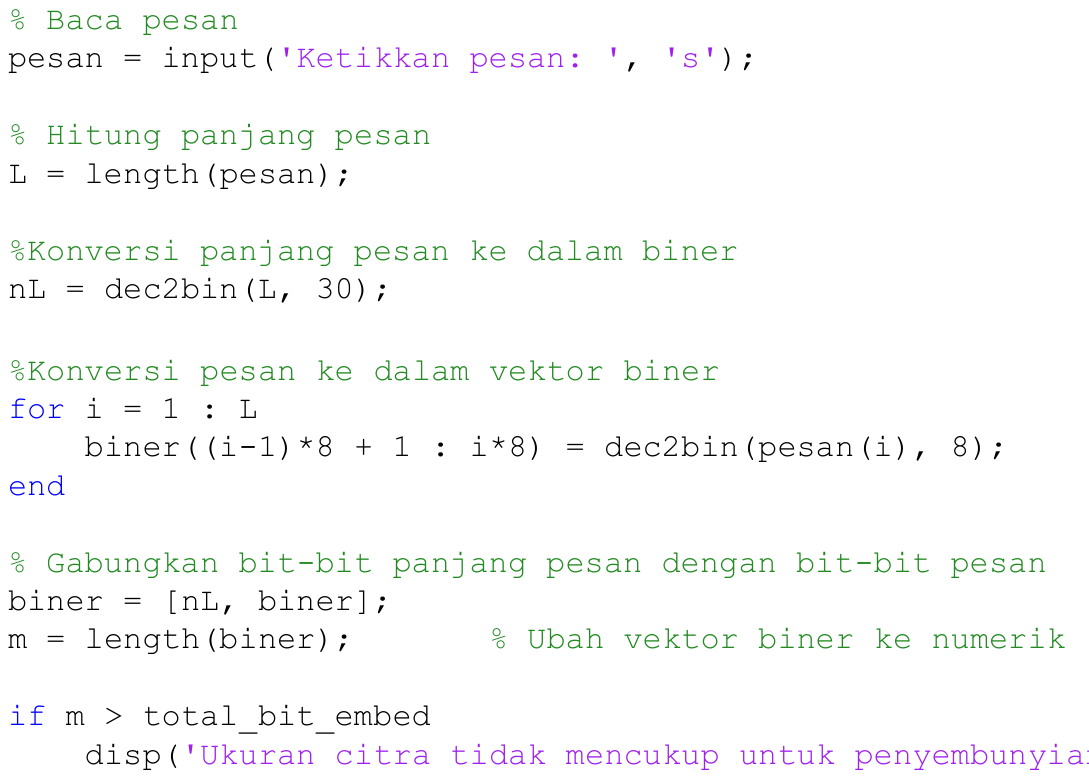
\includegraphics[width=119.07mm,height=213.84mm]{../../images/llm/page_067_img_01.png}%
\end{textblock*}

\end{document}
